\subsubsection{TGDS-Operator}

\classWithoutPage{AlternatingOperator}

\begin{figure}[h]
\centerline{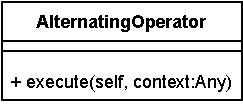
\includegraphics[scale=1]{res/Klassen/AlternatingOperator.pdf}}
\caption{AlternatingOperator class from class diagram}
\end{figure}

This class is a subclass of airflow.models.baseoperator.BaseOperator and is inserted in the plugins folder of the Airflow installation. Then it can be used in the creation of dag-definition-files. The operator takes two tasks and alternates between them. The tasks shall be able to give each other parameters dynamically.

\begin{methodenv}{Methods}

\method{execute(self, context: Any): void}
Overwrites the method execute from it's parent class. This method is called when the operator is used in a workflow. 

\smallPara{Parameters}
\begin{itemize}
	\item{self:}
	The object itself
	\item{context:}
	The airflow context that can be used to read config values
\end{itemize}

\end{methodenv}

\newpage